\hypertarget{mr.-peanut-and-mr.-salty}{%
\section{Mr.~Peanut and Mr.~Salty}\label{mr.-peanut-and-mr.-salty}}

\begin{figure}[!ht]
  \begin{adjustwidth}{-\oddsidemargin-1in}{-\rightmargin}
    \centering
    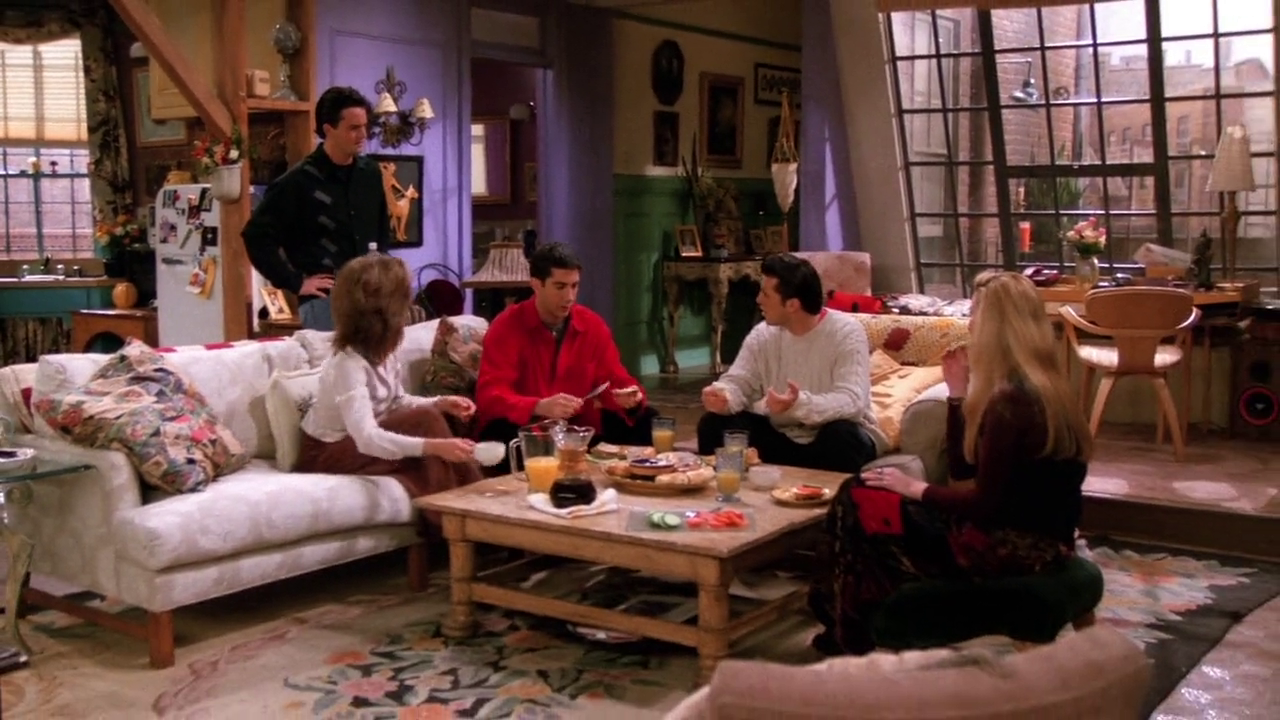
\includegraphics[trim={0 5cm 0 2cm,}, clip, width=\paperwidth]{./S01/img/20/mr-peanut-and-mr-salty.png}
    % \caption{Mr. Peanut and Mr. Salty\label{fig:mr-peanut-and-mr-salty}}
  \end{adjustwidth}
\end{figure}

\begin{tcolorbox}[enhanced,center upper,
    drop fuzzy shadow southeast, boxrule=0.3pt,
    lower separated=false, breakable,
    colframe=black!30!dialogoBorder,colback=white]
\begin{minipage}[c]{0.16\linewidth}
  \raisebox{\dimexpr-\height+\ht\strutbox\relax}{
    \centering 
\includegraphics[width=1.4cm]{./assets/img/chandler.png}
  }
   & \centering \scriptsize{Chandler}
\end{minipage}
\hfill
\begin{minipage}[c]{0.8\linewidth}
  \textbf{- I would much rather be Mr. Peanut than Mr. Salty.}\\
  - Prefiro ser o Sr. Peanut ao ser o Sr. Salty.
\end{minipage}
\end{tcolorbox}

\saveparinfos
\noindent
\begin{minipage}[c]{0.5\textwidth}\useparinfo

Joey e Chandler discutem sobre quem é melhor \emph{Mr.~Peanut} ou
\emph{Mr.~Salty}. Ambos são aperitivos e possuem formas
antropomórficas.\footnote{\sloppy Mr. Peanut - Fandom Wiki. \url{https://mrpeanut.fandom.com/wiki/Mr._Peanut}}

\end{minipage}\hfill
\begin{minipage}[c]{0.5\textwidth}

\begin{figure}
  \centering
  \begin{tikzpicture}
    \node [inner sep=0pt] at (0,0) {
      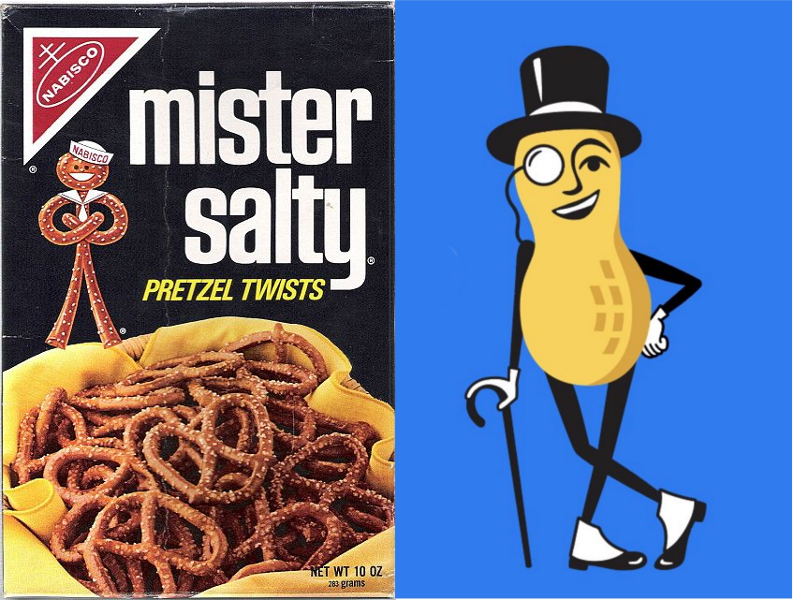
\includegraphics[width=0.8\textwidth,keepaspectratio]{./S01/img/20/mr-peanut-and-mr-salty-chars.png}
    };
    \draw [white, rounded corners=\ClipSep, line width=\ClipSep]
    (current bounding box.north west) --
    (current bounding box.north east) --
    (current bounding box.south east) --
    (current bounding box.south west) -- cycle
    ;
    \end{tikzpicture}
    \caption{Mr. Salty e Mr. Peanut\label{fig:mr-salty-e-mr-peanut}}
\end{figure}

\end{minipage}

\hypertarget{gravity-boots}{%
\section{Gravity Boots}\label{gravity-boots}}

\begin{figure}[!ht]
  \begin{adjustwidth}{-\oddsidemargin-1in}{-\rightmargin}
    \centering
    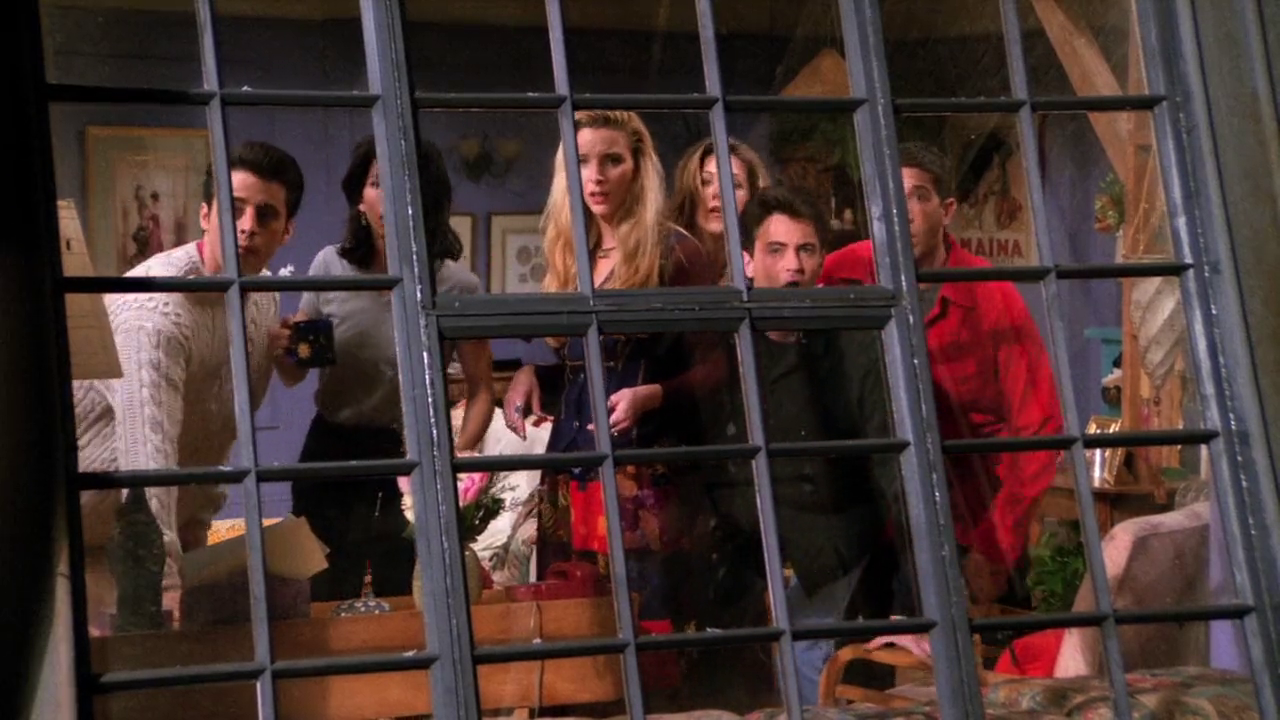
\includegraphics[trim={0 5cm 0 2cm,}, clip, width=\paperwidth]{./S01/img/20/gravity-boots.png}
    % \caption{Gravity Boots\label{fig:gravity-boots}}
  \end{adjustwidth}
\end{figure}

\begin{tcolorbox}[enhanced,center upper,
    drop fuzzy shadow southeast, boxrule=0.3pt,
    lower separated=false, breakable,
    colframe=black!30!dialogoBorder,colback=white]
\begin{minipage}[c]{0.16\linewidth}
  \raisebox{\dimexpr-\height+\ht\strutbox\relax}{
    \centering 
\includegraphics[width=1.4cm]{./assets/img/phoebe.png}
  }
   & \centering \scriptsize{Phoebe}
\end{minipage}
\hfill
\begin{minipage}[c]{0.8\linewidth}
  \textbf{- Oh, you guys, look. Ugly Naked Guy got gravity boots.}\\
  - Olha pessoal. O Peladão feio tem Botas Inversoras.
\end{minipage}
\end{tcolorbox}

\saveparinfos
\noindent
\begin{minipage}[c]{0.5\textwidth}\useparinfo

Phoebe espia o \emph{Peladão feio} e chama os outros para ver que ele
comprou \emph{gravity boots}, que são botas de exercício de abdominal
invertido, ou seja, de cabeça para baixo. Elas possuem ganchos que são
colocados em uma barra fixada.\footnote{\sloppy Inversion Table - WebMD (Inglês). \url{https://www.webmd.com/back-pain/what-are-inversion-tables#3}}

\end{minipage}\hfill
\begin{minipage}[c]{0.5\textwidth}

\begin{figure}
  \centering
  \begin{tikzpicture}
    \node [inner sep=0pt] at (0,0) {
      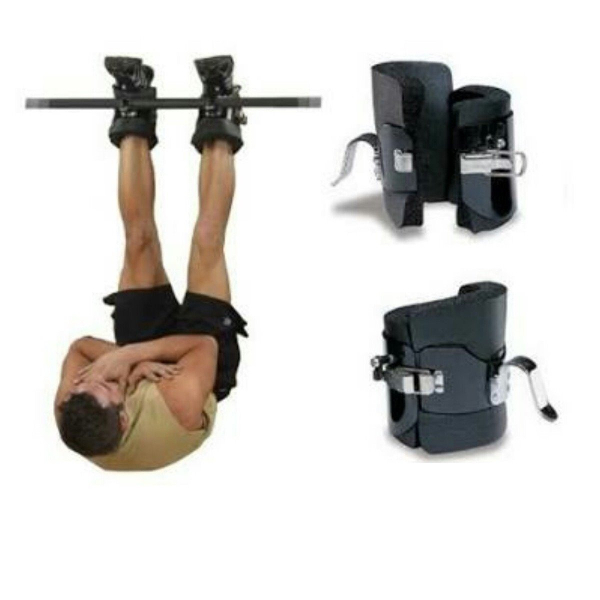
\includegraphics[width=0.8\textwidth,keepaspectratio]{./S01/img/20/gravity-boots-photo.jpg}
    };
    \draw [white, rounded corners=\ClipSep, line width=\ClipSep]
    (current bounding box.north west) --
    (current bounding box.north east) --
    (current bounding box.south east) --
    (current bounding box.south west) -- cycle
    ;
    \end{tikzpicture}
    \caption{Gravity Boots\label{fig:gravity-boots}}
\end{figure}

\end{minipage}

\hypertarget{bendel-and-chanel}{%
\section{Bendel and Chanel}\label{bendel-and-chanel}}

\begin{figure}[!ht]
  \begin{adjustwidth}{-\oddsidemargin-1in}{-\rightmargin}
    \centering
    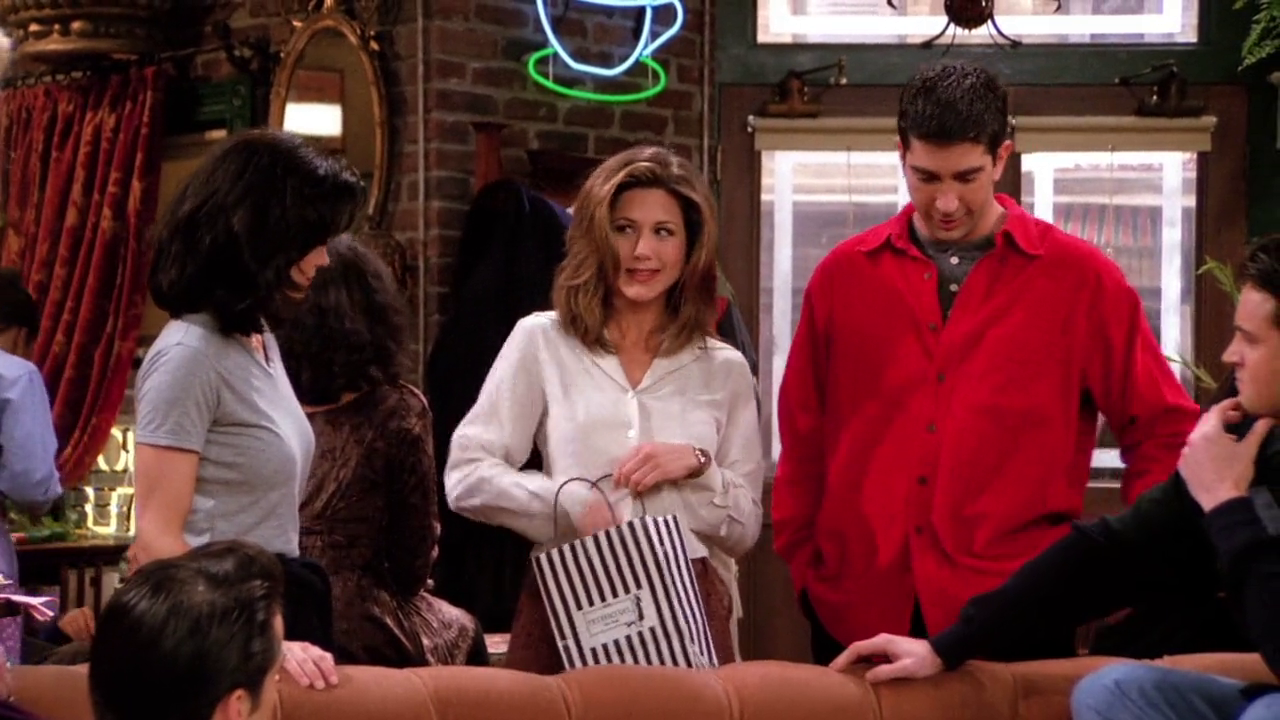
\includegraphics[trim={0 3cm 0 4cm,}, clip, width=\paperwidth]{./S01/img/20/bendel-and-chanel.png}
    % \caption{Bendel and Chanel\label{fig:bendel-and-chanel}}
  \end{adjustwidth}
\end{figure}

\begin{tcolorbox}[enhanced,center upper,
    drop fuzzy shadow southeast, boxrule=0.3pt,
    lower separated=false, breakable,
    colframe=black!30!dialogoBorder,colback=white]
\begin{minipage}[c]{0.16\linewidth}
  \raisebox{\dimexpr-\height+\ht\strutbox\relax}{
    \centering 
\includegraphics[width=1.4cm]{./assets/img/rachel.png}
  }
   & \centering \scriptsize{Rachel}
\end{minipage}
\hfill
\begin{minipage}[c]{0.8\linewidth}
  \textbf{- And then we took a walk to Bendel's. And I told him not to, but he got me a little bottle of Chanel.}\\
  - Fomos até a Bendel's. Falei que não precisava, mas ele me comprou um perfume Chanel.
\end{minipage}
\end{tcolorbox}

Na volta de um encontro com seu ex-noivo Barry, Rachel menciona
\emph{Bendel's} (1895-2019) e \emph{Chanel} (1909-). O primeiro era uma
loja localizada na Quinta Avenida, e que existiu por 123 anos até ser
fechada no começo de 2019. Uma de suas características marcantes era a
sacola de compras, que pode ser vista na mão de Rachel.\footnote{\sloppy Henri Bendel - Exame. \url{https://exame.com/casual/iconica-marca-henri-bendel-fecha-as-portas-apos-123-anos/}}
A segunda refere-se a marca de perfumes e alta-costura fundada pela
estilista francesa \emph{Coco Chanel} (1883-1971).\footnote{\sloppy Coco Chanel- Encyclopædia Britannica. \url{https://www.britannica.com/biography/Coco-Chanel}}
\emph{Henri Bendel} foi o primeiro varejista a vender produtos
\emph{Chanel} nos EUA.

\hypertarget{trouble}{%
\section{Trouble}\label{trouble}}

\begin{figure}[!ht]
  \begin{adjustwidth}{-\oddsidemargin-1in}{-\rightmargin}
    \centering
    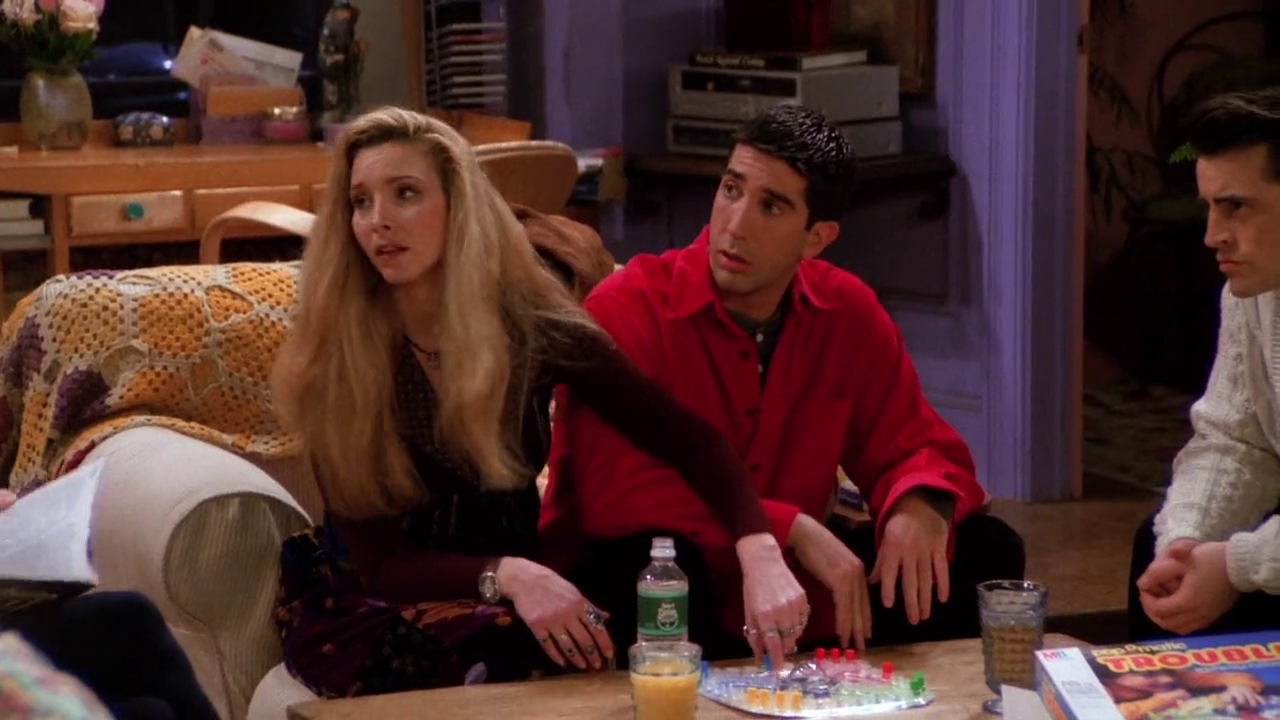
\includegraphics[trim={0 0cm 0 4cm,}, clip, width=\paperwidth]{./S01/img/20/trouble.png}
    % \caption{Trouble\label{fig:trouble}}
  \end{adjustwidth}
\end{figure}

Os amigos jogam uma partida de \emph{Trouble}, conhecido no Brasil como
\emph{Ludo}. Jogo de tabuleiro em que cada jogador possui um conjunto de
peças, que devem se mover uma por rodada com base no lançamento de um
dado. O jogador que mover todas as peças até uma parte central vence o
jogo. Se uma peça cair no mesmo local de uma peça adversária, a mesma é
retornada para o início.\footnote{\sloppy Trouble - Board Game Geek (Inglês). \url{https://www.boardgamegeek.com/boardgame/1410/trouble}}

\begin{figure}
  \centering
  \begin{tikzpicture}
    \node [inner sep=0pt] at (0,0) {
      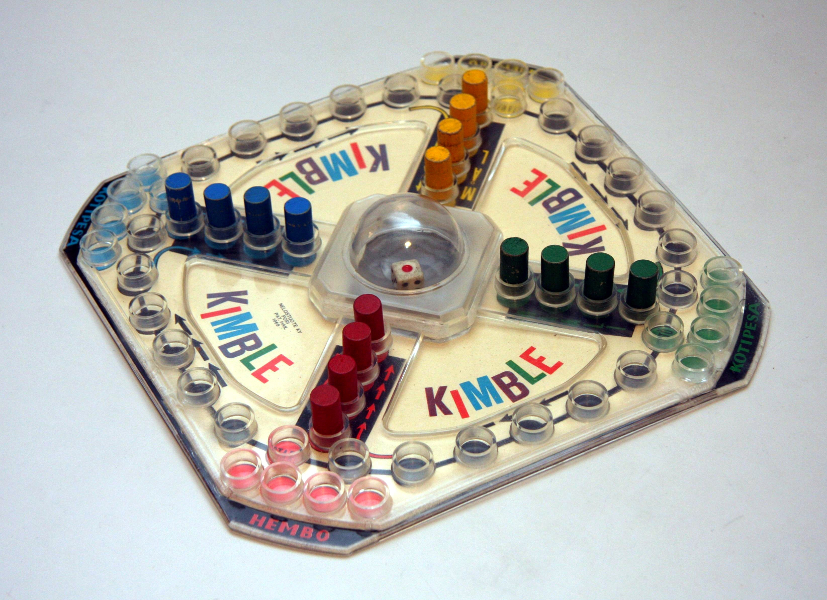
\includegraphics[width=0.5\textwidth,keepaspectratio]{./S01/img/20/trouble-board-game.jpg}
    };
    \draw [white, rounded corners=\ClipSep, line width=\ClipSep]
    (current bounding box.north west) --
    (current bounding box.north east) --
    (current bounding box.south east) --
    (current bounding box.south west) -- cycle
    ;
    \end{tikzpicture}
    \caption{Tabuleiro de Trouble\label{fig:tabuleiro-de-trouble}}
\end{figure}

\hypertarget{get-down-and-boogie}{%
\section{Get down and boogie}\label{get-down-and-boogie}}

\begin{figure}[!ht]
  \begin{adjustwidth}{-\oddsidemargin-1in}{-\rightmargin}
    \centering
    
\includegraphics[trim={0 6cm 0 1cm,}, clip, width=\paperwidth]{./S01/img/20/get-down-and-boogie.png}
    % \caption{Get down and boogie\label{fig:get-down-and-boogie}}
  \end{adjustwidth}
\end{figure}

\begin{tcolorbox}[enhanced,center upper,
    drop fuzzy shadow southeast, boxrule=0.3pt,
    lower separated=false, breakable,
    colframe=black!30!dialogoBorder,colback=white]
\begin{minipage}[c]{0.16\linewidth}
  \raisebox{\dimexpr-\height+\ht\strutbox\relax}{
    \centering 
\includegraphics[width=1.4cm]{./assets/img/joey.png}
  }
   & \centering \scriptsize{Joey}
\end{minipage}
\hfill
\begin{minipage}[c]{0.8\linewidth}
  \textbf{- Get down!}\\
  - Se abaixa!
\end{minipage}

\medskip
\begin{minipage}[c]{0.16\linewidth}
  \raisebox{\dimexpr-\height+\ht\strutbox\relax}{
    \centering 
\includegraphics[width=1.4cm]{./assets/img/rachel.png}
  }
   & \centering \scriptsize{Rachel}
\end{minipage}
\hfill
\begin{minipage}[c]{0.8\linewidth}
  \textbf{- Get down?}\\
  - Se abaixa?
\end{minipage}

\medskip
\begin{minipage}[c]{0.16\linewidth}
  \raisebox{\dimexpr-\height+\ht\strutbox\relax}{
    \centering 
\includegraphics[width=1.4cm]{./assets/img/chandler.png}
  }
   & \centering \scriptsize{Chandler}
\end{minipage}
\hfill
\begin{minipage}[c]{0.8\linewidth}
  \textbf{- And boogie!}\\
  - Até o chão!
\end{minipage}
\end{tcolorbox}

Chandler refere-se a um termo proviniente de um estilo popular de
\emph{blues} dos anos 30, mas que foi mais difundido para descrever os
estilos \emph{rock} sulista e \emph{disco music}.\footnote{\sloppy Various ‎- Get Down And Boogie - Discogs. \url{https://www.discogs.com/pt_BR/Various-Get-Down-And-Boogie/release/98158}}
\footnote{\sloppy Name it on the `boogie' - the genre tag that won’t sit still - The Guardian (Inglês). \url{https://www.theguardian.com/music/musicblog/2011/may/03/simon-reynolds-boogie-genre-term}}
Em 1976 foi lançada a coletânea \emph{Get Down And Boogie}, que incluía
a música \emph{Love To Love You Baby} de \emph{Donna Summer}, que
aparece no episódio
\textbf{\textcolor{primarycolor}{S05E23 - Aquele em Vegas: Parte 1}}.

\hypertarget{ingrid-bergman}{%
\section{Ingrid Bergman}\label{ingrid-bergman}}

\begin{figure}[!ht]
  \begin{adjustwidth}{-\oddsidemargin-1in}{-\rightmargin}
    \centering
    
\includegraphics[trim={0 5cm 0 2cm,}, clip, width=\paperwidth]{./S01/img/20/ingrid-bergman.png}
    % \caption{Ingrid Bergman\label{fig:ingrid-bergman}}
  \end{adjustwidth}
\end{figure}

\begin{tcolorbox}[enhanced,center upper,
    drop fuzzy shadow southeast, boxrule=0.3pt,
    lower separated=false, breakable,
    colframe=black!30!dialogoBorder,colback=white]
\begin{minipage}[c]{0.16\linewidth}
  \raisebox{\dimexpr-\height+\ht\strutbox\relax}{
    \centering 
\includegraphics[width=1.4cm]{./assets/img/joey.png}
  }
   & \centering \scriptsize{Joey}
\end{minipage}
\hfill
\begin{minipage}[c]{0.8\linewidth}
  \textbf{- Yeah, my neighbor... Yeah, the brunette... She says you looked very pretty the other day in the green dress.}\\
  - Sim, minha vizinha... Sim, a morena... Ela diz que você estava muito bonita outro dia com aquele vestido verde.
\end{minipage}

\medskip
\begin{minipage}[c]{0.16\linewidth}
  \raisebox{\dimexpr-\height+\ht\strutbox\relax}{
    \centering 
\includegraphics[width=1.4cm]{./assets/img/monica.png}
  }
   & \centering \scriptsize{Monica}
\end{minipage}
\hfill
\begin{minipage}[c]{0.8\linewidth}
  \textbf{- The green dress? Really?}\\
  - O vestido verde? Sério?
\end{minipage}

\medskip
\begin{minipage}[c]{0.16\linewidth}
  \raisebox{\dimexpr-\height+\ht\strutbox\relax}{
    \centering 
\includegraphics[width=1.4cm]{./assets/img/joey.png}
  }
   & \centering \scriptsize{Joey}
\end{minipage}
\hfill
\begin{minipage}[c]{0.8\linewidth}
  \textbf{- Yeah, she said you looked like Ingrid Bergman that day.}\\
  - Sim, ela disse que você parecia a Ingrid Bergman.
\end{minipage}

\medskip
\begin{minipage}[c]{0.16\linewidth}
  \raisebox{\dimexpr-\height+\ht\strutbox\relax}{
    \centering 
\includegraphics[width=1.4cm]{./assets/img/monica.png}
  }
   & \centering \scriptsize{Monica}
\end{minipage}
\hfill
\begin{minipage}[c]{0.8\linewidth}
  \textbf{- Nooo!}\\
  - Nãoo!
\end{minipage}
\end{tcolorbox}

Joey reclama pelo telefone com a vizinha da frente, Sidney, que estava
bisbilhotando os amigos com um telescópio. Entretanto ela reverte a
situação fazendo elogios a Monica, e a compara com \emph{Ingrid Bergman}
(1915-1982), atriz sueca que estrelou, entre outros, o filme
\emph{Casablanca} (1942).\footnote{\sloppy Ingrid Bergman - IMDB. \url{https://www.imdb.com/name/nm0000006/}}
\footnote{\sloppy Ingrid Bergman - Encyclopædia Britannica. \url{https://www.britannica.com/biography/Ingrid-Bergman}}
